\section{Architecture}
The architecture of Doom engine is a complete departure from Wolfenstein 3D. id had to come up with a system allowing to develop on NextStep and build on MS-DOS with as little friction as possible. The solution they came up with was to have a "kernel" common to all platforms tapping into sub-systems specific to the hardware they supported.\\
\par
\begin{figure}[H]
\centering
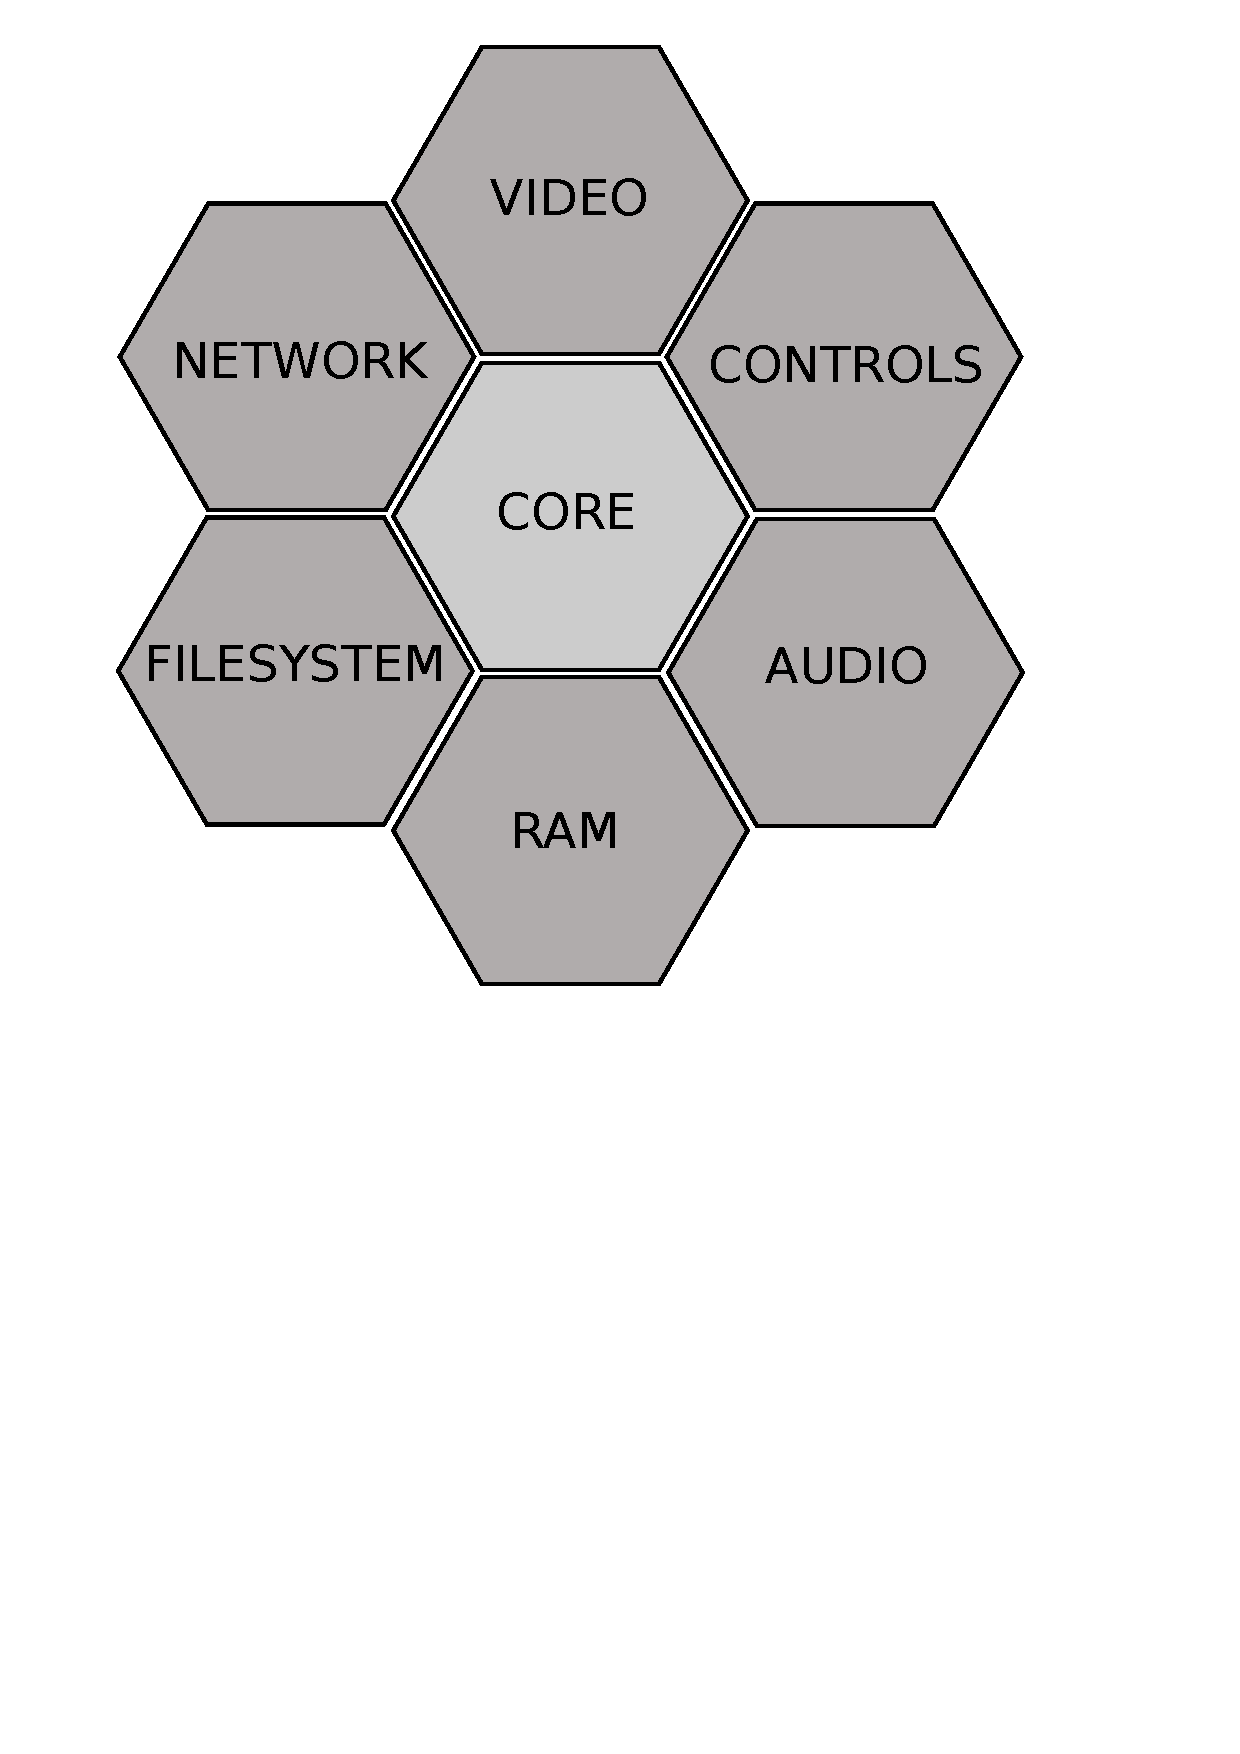
\includegraphics[width=.5\textwidth]{drawings/doom_arch.pdf}
\caption{Doom kernel and its I/O platform-dependent systems.}
\end{figure}
\par
The kernel six sub-systems are:\\
\par
\begin{enumerate}
\item
\item
\item
\item
\item
\item
\end{enumerate}
To implement this system, they exploited the C language ability to declare in a header file (\cw{.h}) a library interface that will only be available later. Each components, the core and all systems for the target plateform are compiled independently during a first step. The C linker combine all object files into an executable (in the case of MS-DOS \cw{DOOM.EXE}).\\
\par
TODO, example with kernel.c, video.h, audio.h. video.c and audio.c.\\ 
\par
Doom ASM improved performances by 16\%. Detail here the method (timedemo) and realtick. FPS 14 to 16.\\
\par


\par

\trivia{
Doom build time\\ 
Full build = 9:37 (among it: 19s to link)\\
Partial build (r\_sky.c) = 27s (among it 19s to link).\\}
\par

Abstraction layer (compare VGA in wolf3d to doom) incured small overhead but also unlocked new algorithm and allowed easy port -> even a fridge runs doom.\\
\par
NextStep dithering.\\
\\ 

\trivia{The MS-DOS source code features what should have been a Doom easter egg. Files \cw{am\_oids.h} and \cw{am\_oids.c} were to allow player to play a remake of Asteroids in the automap but was left unfinished.}\\
\par
\fq{I can’t recall whose idea it was, but it was probably mine.  I was taken by the vector art style of the automap, so Asteroids would have been a good fit, but Doom was behind, and the pace of development at id was incredibly fast.}{Dave Taylor}
\tcode{cloc.txt}


\fullimage{Doom_build_NeXTStep.png}

\trivia{What are the dot during startup?}

\section{Structure of the code}
The kernel is made of 45 translation units and is common to all version of \doom.\\
\par

\drawing{doom_code_arch}{}
\par

The I/O system differ on DOS and \NeXT.\\
\par

 \begin{figure}[H]
\centering  
\begin{tabularx}{\textwidth}{ L{0.4} L{0.6} }
  \toprule
  \textbf{Filename} & \textbf{Description}\\
  \toprule 
   i\_main.c & \\
i\_ibm.c  & \\
planar.asm    & \\    
i\_ibm\_a.asm & \\
i\_sound.c & \\
i\_cyber.c & \\
   \toprule
\end{tabularx}
\caption{DOS specific code}
\end{figure}

\par


 \begin{figure}[H]
\centering  
\begin{tabularx}{\textwidth}{ L{0.4} L{0.6} }
  \toprule
  \textbf{Filename} & \textbf{Description}\\
  \toprule 
DRCoord.m  & \\
VGAView.m & \\
fpfunc.s & \\
Doom\_main.m  & \\
i\_next.m  & \\
r\_debug.m & \\
   \toprule
\end{tabularx}
\caption{NeXT specific code}
\end{figure}

Some systems are bigger than others. Since it is basd on \cw{<stdio.h>}, the filesystem is very tiny and takes care of the difference in endianess
